\documentclass[12pt,a4paper]{article}
\usepackage[utf8]{inputenc}
\usepackage{tabularx}
\usepackage{spverbatim}
\usepackage{listings}
\usepackage{placeins}
\usepackage{mainpackage}

\begin{document}

\begin{titlepage}
    \centering
    \vspace*{\fill}

    \vspace*{0.5cm}

    \huge
    TDT4145 - Øving 3

    \vspace*{0.5cm}

    \large Sander Lindberg

    \vspace*{\fill}
    \end{titlepage}

	\newpage

	\section{Oppgave 1}
	\subsection{a}
		Dette kan gjøres med ON DELETE CASCADE
	
	\subsection{b}
		\begin{spverbatim}
USE film;

CREATE TABLE regissør(
regissørID INTEGER NOT NULL,
navn VARCHAR(255),
 CONSTRAINT regissør_PK PRIMARY KEY (regissørID)
);

CREATE TABLE film (
filmID INTEGER NOT NULL,
title VARCHAR(30),
prodaar INTEGER,
regissorID INTEGER NOT NULL,
CONSTRAINT film_PK PRIMARY KEY (filmID),
CONSTRAINT film_FK FOREIGN KEY (regissorID)
	REFERENCES regissør (regissørID),
CONSTRAINT aarsjekk CHECK (prodaar < YEAR(GETDATE()))
);

CREATE TABLE sjanger (
sjangerID INTEGER NOT NULL,
navn VARCHAR(20) NOT NULL,
beskrivelse VARCHAR(255),
CONSTRAINT sjanger_PK PRIMARY KEY (sjangerID)
);

CREATE TABLE sjangerforfilm (
filmID INTEGER NOT NULL,
sjangerID INTEGER NOT NULL,
CONSTRAINT sjangerforfilm_PK PRIMARY KEY (filmID, sjangerID),
CONSTRAINT sjangerforfilm_FK1 FOREIGN KEY (filmID) REFERENCES film (filmID) ON DELETE CASCADE,
CONSTRAINT sjangerforfilm_FK2 FOREIGN KEY (sjangerID) REFERENCES sjanger (sjangerID)
);

CREATE TABLE skuespiller (
skuespillerID INTEGER NOT NULL,
navn VARCHAR(255),
faar INTEGER NOT NULL,
CONSTRAINT skuespiller_PK PRIMARY KEY (skuespillerID),
CONSTRAINT aarsjekk CHECK (faar < YEAR(getdate()))
);

CREATE TABLE skuespillerifIlm (
filmID INTEGER NOT NULL,
skuespillerID INTEGER NOT NULL,
rolle VARCHAR(255),
CONSTRAINT skuespillerifilm_PK PRIMARY KEY (filmID, skuespillerID),
CONSTRAINT skuespillerifilm_FK1 FOREIGN KEY (filmID) REFERENCES film (filmID) ON DELETE CASCADE,
CONSTRAINT skuespillerifilm_FK2 FOREIGN KEY (skuespillerID) REFERENCES skuespiller (skuespillerID)
);
	\end{spverbatim}
	
	\subsection{c}
	\begin{spverbatim}	
INSERT INTO regissør VALUES (1, "Python Reed"), (2, "Tom Shadyac");

INSERT INTO film VALUES (1, "Yes Man", 2008, 1);

INSERT INTO skuespiller VALUES (1 , "Jim Carrey", 1962);

INSERT INTO skuespillerifilm VALUES (1, 1, "Carl")	
	\end{spverbatim}
	
	\subsection{d}
	\begin{spverbatim}
UPDATE skuespiller SET navn = "James Eugene Carrey" WHERE skuespillerID = 1;
	\end{spverbatim}	
	
	\subsection{e}
	\begin{spverbatim}
DELETE FROM regissør where regissørID = 2;
	\end{spverbatim}	
	
	\section{Oppgave 2}
	\subsection{a}
	\begin{spverbatim}
SELECT * FROM film;
	\end{spverbatim}	
	
	\subsection{b}
	\begin{spverbatim}
SELECT navn FROM skuespiller where faar > 1960;
	\end{spverbatim}	
	
	\subsection{c}
	\begin{spverbatim}
SELECT * FROM skuespiller WHERE faar BETWEEN 1980 AND 1989 ORDER BY navn ASC;
	\end{spverbatim}	
	
	\subsection{d}
	\begin{spverbatim}
SELECT film.title, skuespillerifilm.rolle FROM film 
JOIN skuespillerifilm ON film.filmID = skuespillerifilm.filmID 
JOIN skuespiller ON skuespiller.skuespillerID = skuespillerifIlm.skuespillerID 
WHERE navn = "Morgan Freeman";
	\end{spverbatim}	
	
	\subsection{e}
	\begin{spverbatim}
SELECT DISTINCT  title 
FROM film 
JOIN regissør ON film.regissorID = regissør.regissørID J
OIN skuespillerifIlm ON film.filmID = skuespillerifilm.filmID 
JOIN skuespiller ON skuespillerifilm.skuespillerID = skuespiller.skuespillerID
WHERE skuespiller.navn = regissør.navn;
	\end{spverbatim}	
	
	\subsection{f}
	\begin{spverbatim}
SELECT DISTINCT COUNT(navn) as 'Antall_navn_c' FROM skuespiller WHERE navn LIKE "C%";
	\end{spverbatim}	
	
	\subsection{g}
	\begin{spverbatim}
SELECT DISTINCT sjanger.navn, COUNT(film.filmID)
FROM sjangerforfilm
JOIN film ON sjangerforfilm.filmID = film.filmID 
JOIN sjanger ON sjangerforfilm.sjangerID = sjanger.sjangerID
GROUP BY sjanger.navn; 
	\end{spverbatim}
	
	\subsection{h}
	\begin{spverbatim}
SELECT skuespiller.navn
FROM skuespiller JOIN skuespillerifilm ON skuespiller.skuespillerID 
= skuespillerifilm.skuespillerID
JOIN film ON film.filmID = skuespillerifilm.filmID
WHERE film.title = "Ace Ventura: Pet Detective" 
AND skuespiller.skuespillerID NOT IN (
SELECT skuespiller.skuespillerID
FROM skuespiller JOIN skuespillerifilm ON skuespiller.skuespillerID 
= skuespillerifilm.skuespillerID
JOIN film ON film.filmID = skuespillerifilm.filmID
WHERE film.title = "Ace Ventura: When Nature Calls");
	\end{spverbatim}	
	
	\subsection{i}
	\begin{spverbatim}
SELECT film.title, AVG(skuespiller.faar) AS Average_age_movie
FROM film JOIN skuespillerifilm ON skuespillerifilm.filmID = film.filmID
JOIN skuespiller ON skuespiller.skuespillerID = skuespillerifilm.skuespillerID
GROUP BY film.filmID
HAVING Average_age_movie > 
(SELECT AVG(skuespiller.faar) FROM film JOIN skuespillerifilm
ON skuespillerifilm.filmID = film.filmID
JOIN skuespiller ON skuespiller.skuespillerID = skuespillerifilm.skuespillerID);
	\end{spverbatim}	
	
	\section{Oppgave 3}
	\begin{figure}[!ht]
		\centering
		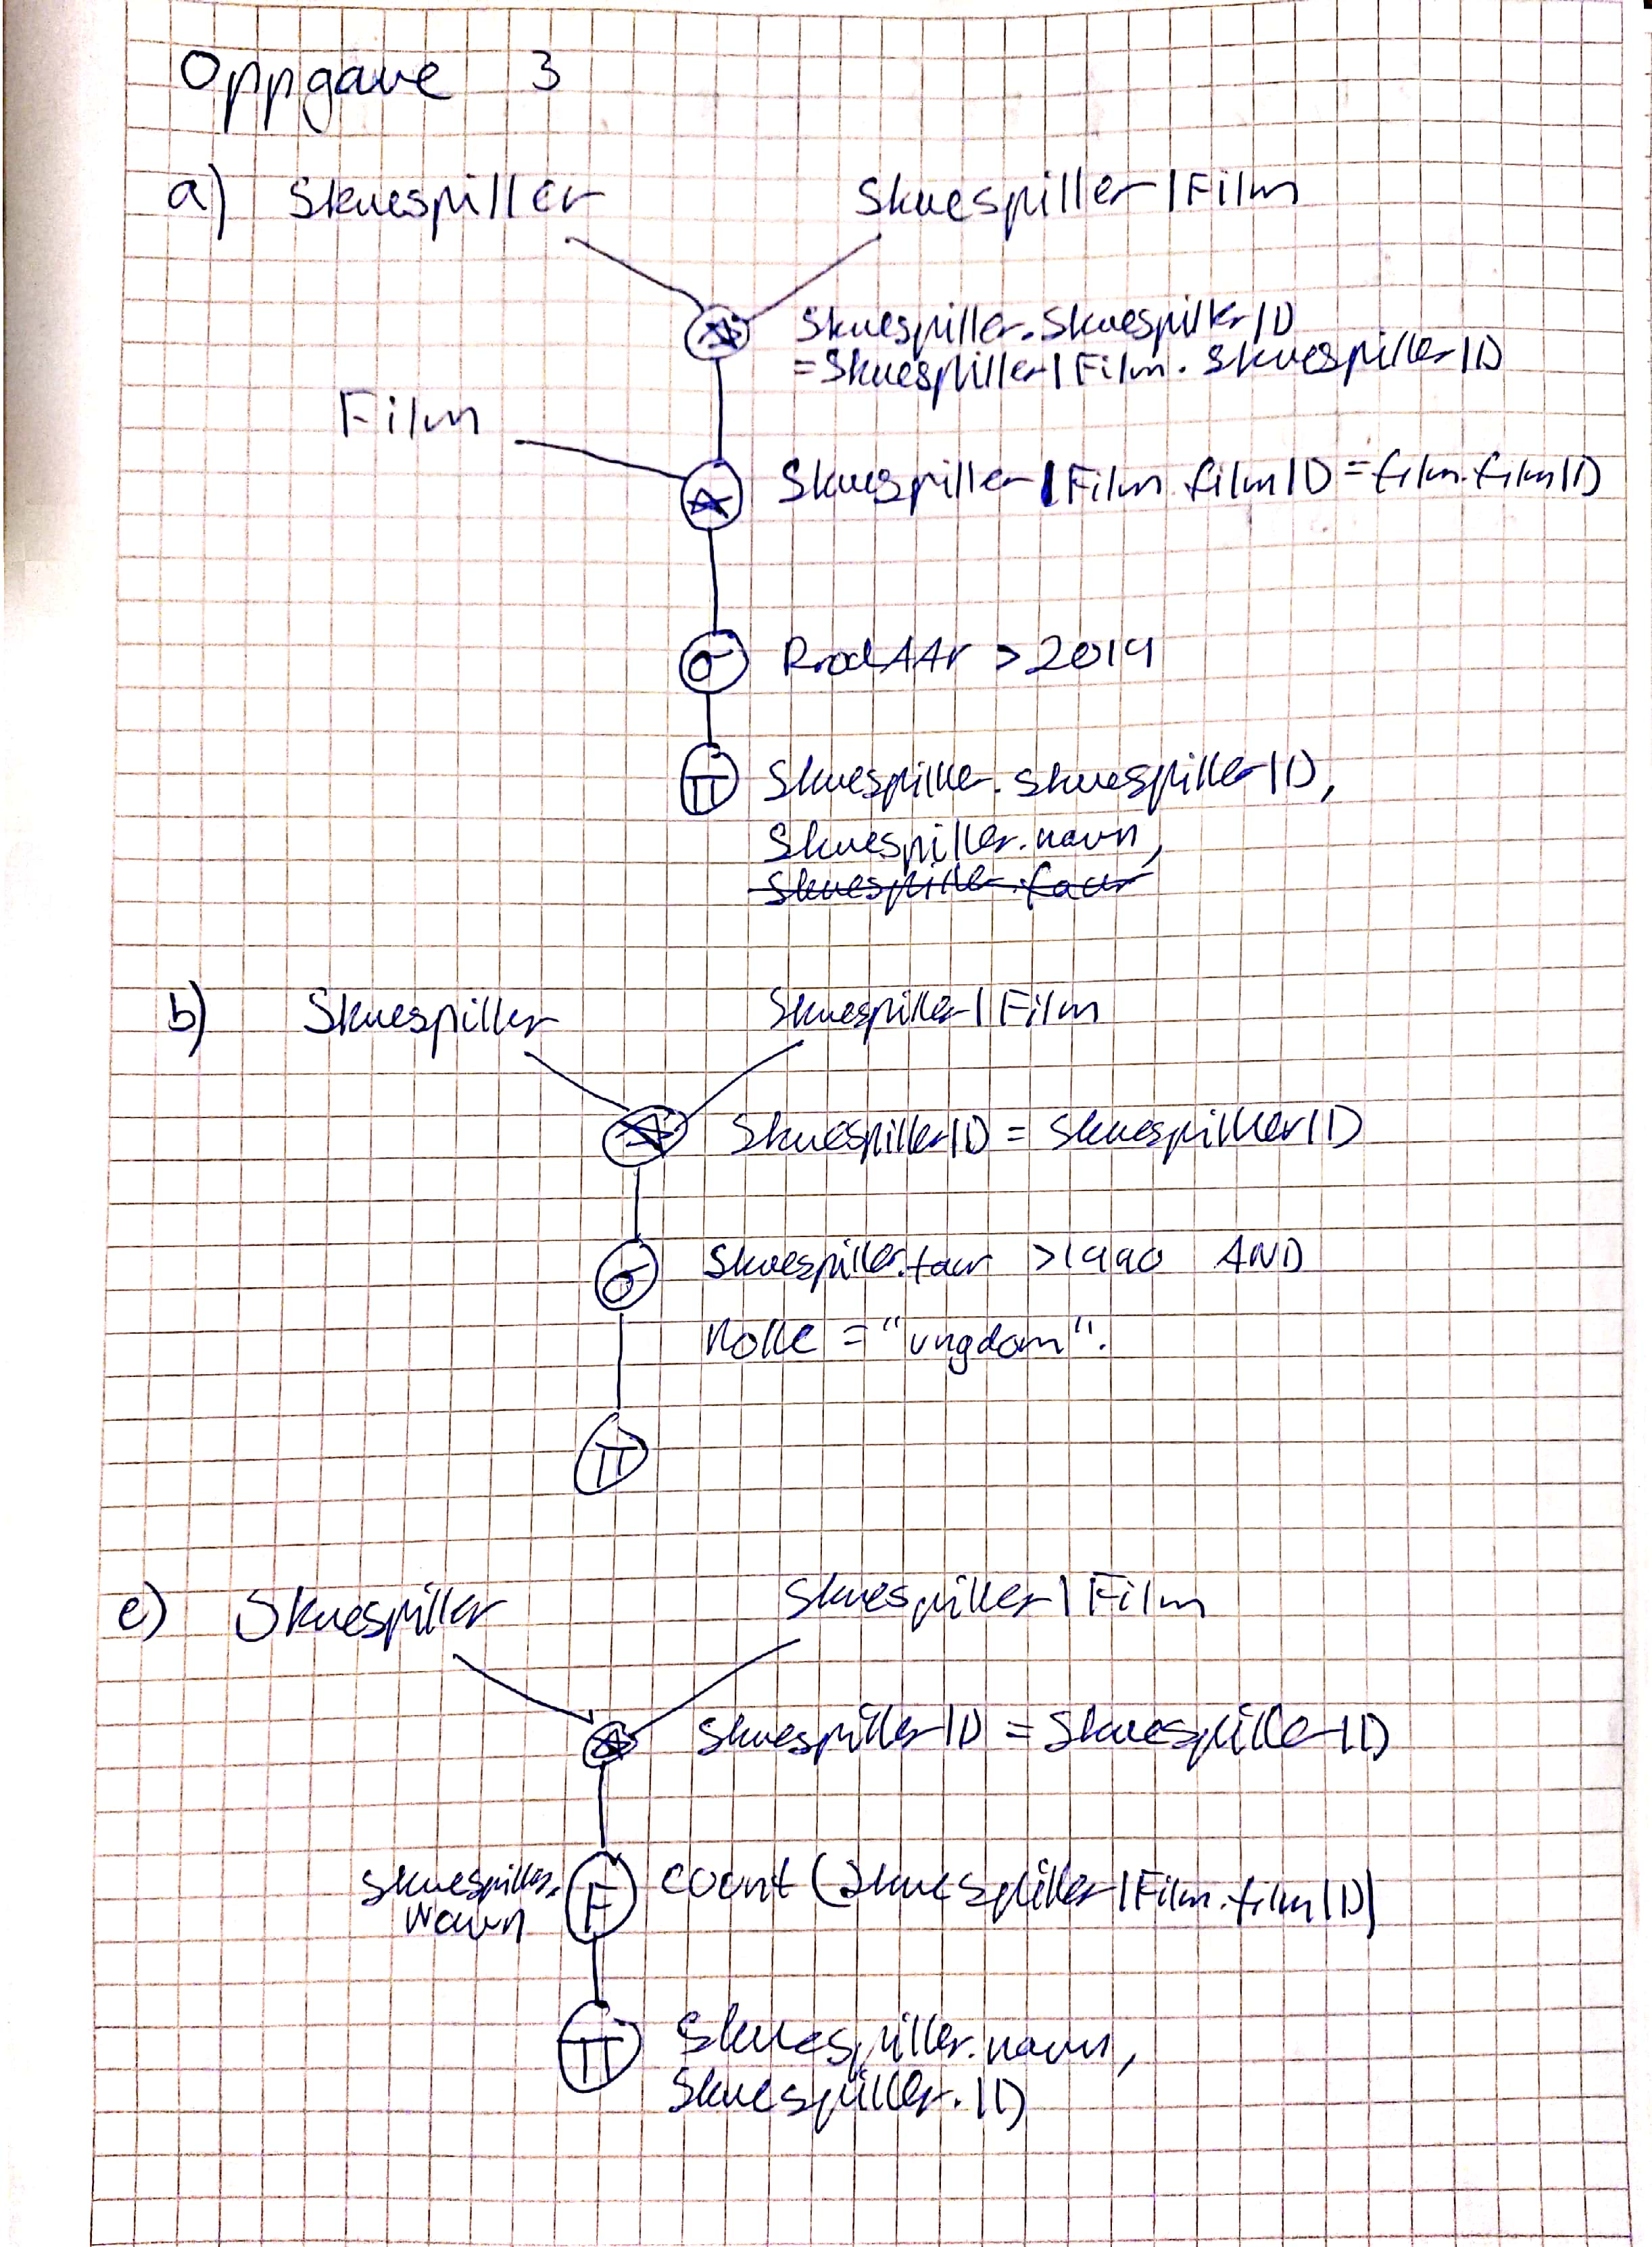
\includegraphics[width=\linewidth]{oppgave_3_oving_3.jpg}
		\caption{Oppgave 3 - Relasjonsalgebra}
		\label{fig:oppgave_3}
	\end{figure}		
	\FloatBarrier
	\section{Oppgave 4}
	\subsection{a}
		3 rader, 15 kolonner.
	
	\subsection{b}
		Ville satt fakultet i en egen tabell:
		
		Fakultet(\underline{fakultetkode}, fakultetsnavn, fakultetsbygg)
		
		Og ansatt i en annen:
		
		Ansatt(\underline{PersonID}, Navn, Telefonnr, \underline{fakultetkode})
		
		Her har jeg satt fakultetkode i ansatttabellen, da en ansatt kan kun ha et fakultet, mens fakulteter kan ha flere ansatte.
		
	\section{Oppgave 4}
	\subsection{a}
		\begin{enumerate}
			\item Ja
			\item Kan kanskje stemme, da alle a'er peker på unike verdier av $b1$. Altså, $a_1$ peker kun på $b_1$, $a_2$ peker kun på $b_1$ osv\dots Vet ikke om dette er tilfelle i ''resten'' av tabellen.
			\item Nei. $a_1$ peker på både $c_1$ og $c_2$.
			\item Nei, $a_1b_1$ peker på $c_1$ og $c_2$.
			\item Kanskje, samme som 2)
			\item Nei. $d_2$ peker både på $c_2$ og $c_4$
			\item Ja $a \rightarrow a$, $b \rightarrow b$, $c \rightarrow c$, $d \rightarrow d$
			\item Kanskje. Gitt at $c \rightarrow d$ stemmer. 
			\item Nei, $a_1$ f.eks identfiserer to rader.
			\item Kanskje, vi kan komme oss til $ABCD$ ved hjelp av $AC$.
		\end{enumerate}
		
	\subsection{b}
		$R = \{A, B, C, D\}$, $F = \{A \rightarrow C, B \rightarrow D, ABC \rightarrow D \}$:
		
		$A^+ = AC$
		
		$D^+ = D$
		
		$BC^+ = BCD$
		
		$AB^+ = ABCD$	
		 
\end{document} 